\documentclass{beamer}

\usecolortheme[dark,accent=cyan]{solarized}

\beamertemplatenavigationsymbolsempty

\usepackage{graphicx}
\usepackage{hyperref}
\usepackage{colortbl, xcolor}
\usepackage{booktabs}

\definecolor{DarkGray}{gray}{0.1}
\definecolor{DarkGray}{gray}{0.1}

\usepackage{tikz}
\usetikzlibrary{calc}
\usepackage{amsmath} % a package for building a matrix
\usetikzlibrary{plotmarks} % a package for building line plots using defined data sets
\usepackage{pgfplots}

\usepackage{enumitem} % a package for the symbols in an itemize

% For code illustration
\usepackage{listing}
\usepackage{minted}
\usemintedstyle{native}
\title{Prisoners and Spatial Structure}
\author{@NikoletaGlyn}
\date{}
\institute[]
{
\begin{center}
    
\includegraphics[width=.15\textwidth]{static/pycon-namibia.png}
\end{center}}

\begin{document}

\frame{\titlepage}

\begin{frame}{Prisoners and Spatial Structure}
 \Huge
 \[
\begin{bmatrix}
  (3,3) & (0,5)  \\
  (5,0) & (1,1)
\end{bmatrix}
\]
\end{frame}

\begin{frame}[fragile]{Strategy}
	\begin{center}
		\begin{minipage}{0.8\textwidth}
			\begin{minted}
[
frame=lines,
framesep=2mm,
baselinestretch=1.2,
fontsize=\tiny,
bgcolor=DarkGray,
linenos
]
{python}

class Grumpy(Player):
    """
    A player that gets grumpier the more the opposition defects,
    and nicer the more they cooperate. Starts off Nice, but becomes
    grumpy once the grumpiness threshold is hit. Won't become nice
    once that grumpy threshold is hit, but must reach a much
    lower threshold before it becomes nice again.
    """

    self.grumpiness = opponent.defections - opponent.cooperations

    if self.state == 'Nice':
        if self.grumpiness > self.grumpy_threshold:
            self.state = 'Grumpy'
            return D
        return C

    if self.state == 'Grumpy':
        if self.grumpiness < self.nice_threshold:
            self.state = 'Nice'
            return C
         return D
			\end{minted}
		\end{minipage}
	\end{center}
\end{frame}


\begin{frame}{History Line}
\def\labellist{{" ","(1980)","(1991)","(1992)","(2012)"," ","(2015)"," "}}
    \begin{tikzpicture}
            \begin{axis}[
                height=8cm,
                width=12cm,
                axis lines=left,
                xtick=\empty,
                ytick=\empty,
                nodes near coords={
                                    \pgfmathparse{\labellist[\coordindex]}%
                                    \pgfmathresult }
                ]
    \addplot[color=white,mark=x]
        coordinates{
            (1,1)
            (2,1.1)
            (3,6)
            (4,6.5)
            (5,8.5)
            (6,9)
            (7,9.5)
            (8,12) };
            \end{axis}
    \end{tikzpicture}
\end{frame}

\begin{frame}{Nowak and May, 1992}
    \begin{center}
        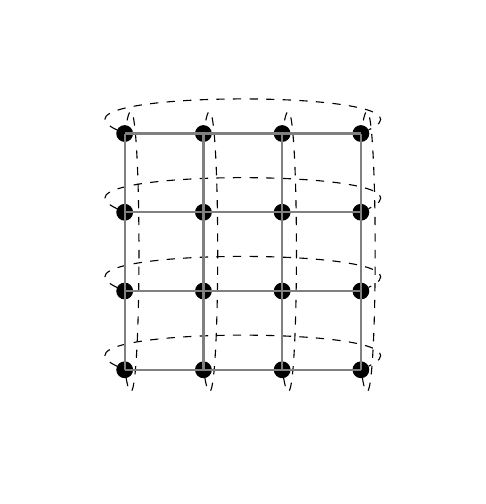
\begin{tikzpicture}
                % First column (tikz has the ability to use loops but I'm drawing it
                % this way so you see how.
                \node (00) [draw, circle, inner sep=2pt,fill] at (0, 0) {};
                \node (01) [draw, circle, inner sep=2pt,fill] at (0, 1) {};
                \node (02) [draw, circle, inner sep=2pt,fill] at (0, 2) {};
                \node (03) [draw, circle, inner sep=2pt,fill] at (0, 3) {};

                % Second column
                \node (10) [draw, circle, inner sep=2pt,fill] at (1, 0) {};
                \node (11) [draw, circle, inner sep=2pt,fill] at (1, 1) {};
                \node (12) [draw, circle, inner sep=2pt,fill] at (1, 2) {};
                \node (13) [draw, circle, inner sep=2pt,fill] at (1, 3) {};

                % Third column
                \node (20) [draw, circle, inner sep=2pt,fill] at (2, 0) {};
                \node (21) [draw, circle, inner sep=2pt,fill] at (2, 1) {};
                \node (22) [draw, circle, inner sep=2pt,fill] at (2, 2) {};
                \node (23) [draw, circle, inner sep=2pt,fill] at (2, 3) {};

                % Fourth column
                \node (30) [draw, circle, inner sep=2pt,fill] at (3, 0) {};
                \node (31) [draw, circle, inner sep=2pt,fill] at (3, 1) {};
                \node (32) [draw, circle, inner sep=2pt,fill] at (3, 2) {};
                \node (33) [draw, circle, inner sep=2pt,fill] at (3, 3) {};


                % I am drawing the periodic boundaries before the rest of the grid
                % so that they appear 'behind' the rest of the images.
                % Draw the period horizontal boundary
                \draw[dashed] (00) to[out=155,in=25 ] (30);
                \draw[dashed] (01) to[out=155,in=25 ] (31);
                \draw[dashed] (02) to[out=155,in=25 ] (32);
                \draw[dashed] (03) to[out=155,in=25 ] (33);

                % Draw the period vertical boundary
                \draw[dashed] (00) to[out=-80,in=80] (03);
                \draw[dashed] (10) to[out=-80,in=80] (13);
                \draw[dashed] (20) to[out=-80,in=80] (23);
                \draw[dashed] (30) to[out=-80,in=80] (33);

                % Draw a grid (this is a tikz shortcut)
                \draw[style=help lines,thick] (0,0) grid  (3,3);
        \end{tikzpicture}
    \end{center}
\end{frame}

\begin{frame}{What do real life interactions look like?}
\begin{center}
		\includegraphics[width=0.8\linewidth]{static/network_no_labels.pdf}
\end{center}
\end{frame}

\begin{frame}{What do real life interactions look like?}
\begin{center}
		\includegraphics[width=0.8\linewidth]{static/network_with_labels.pdf}
\end{center}
\end{frame}

\begin{frame}{Measurements}
	\begin{center}
		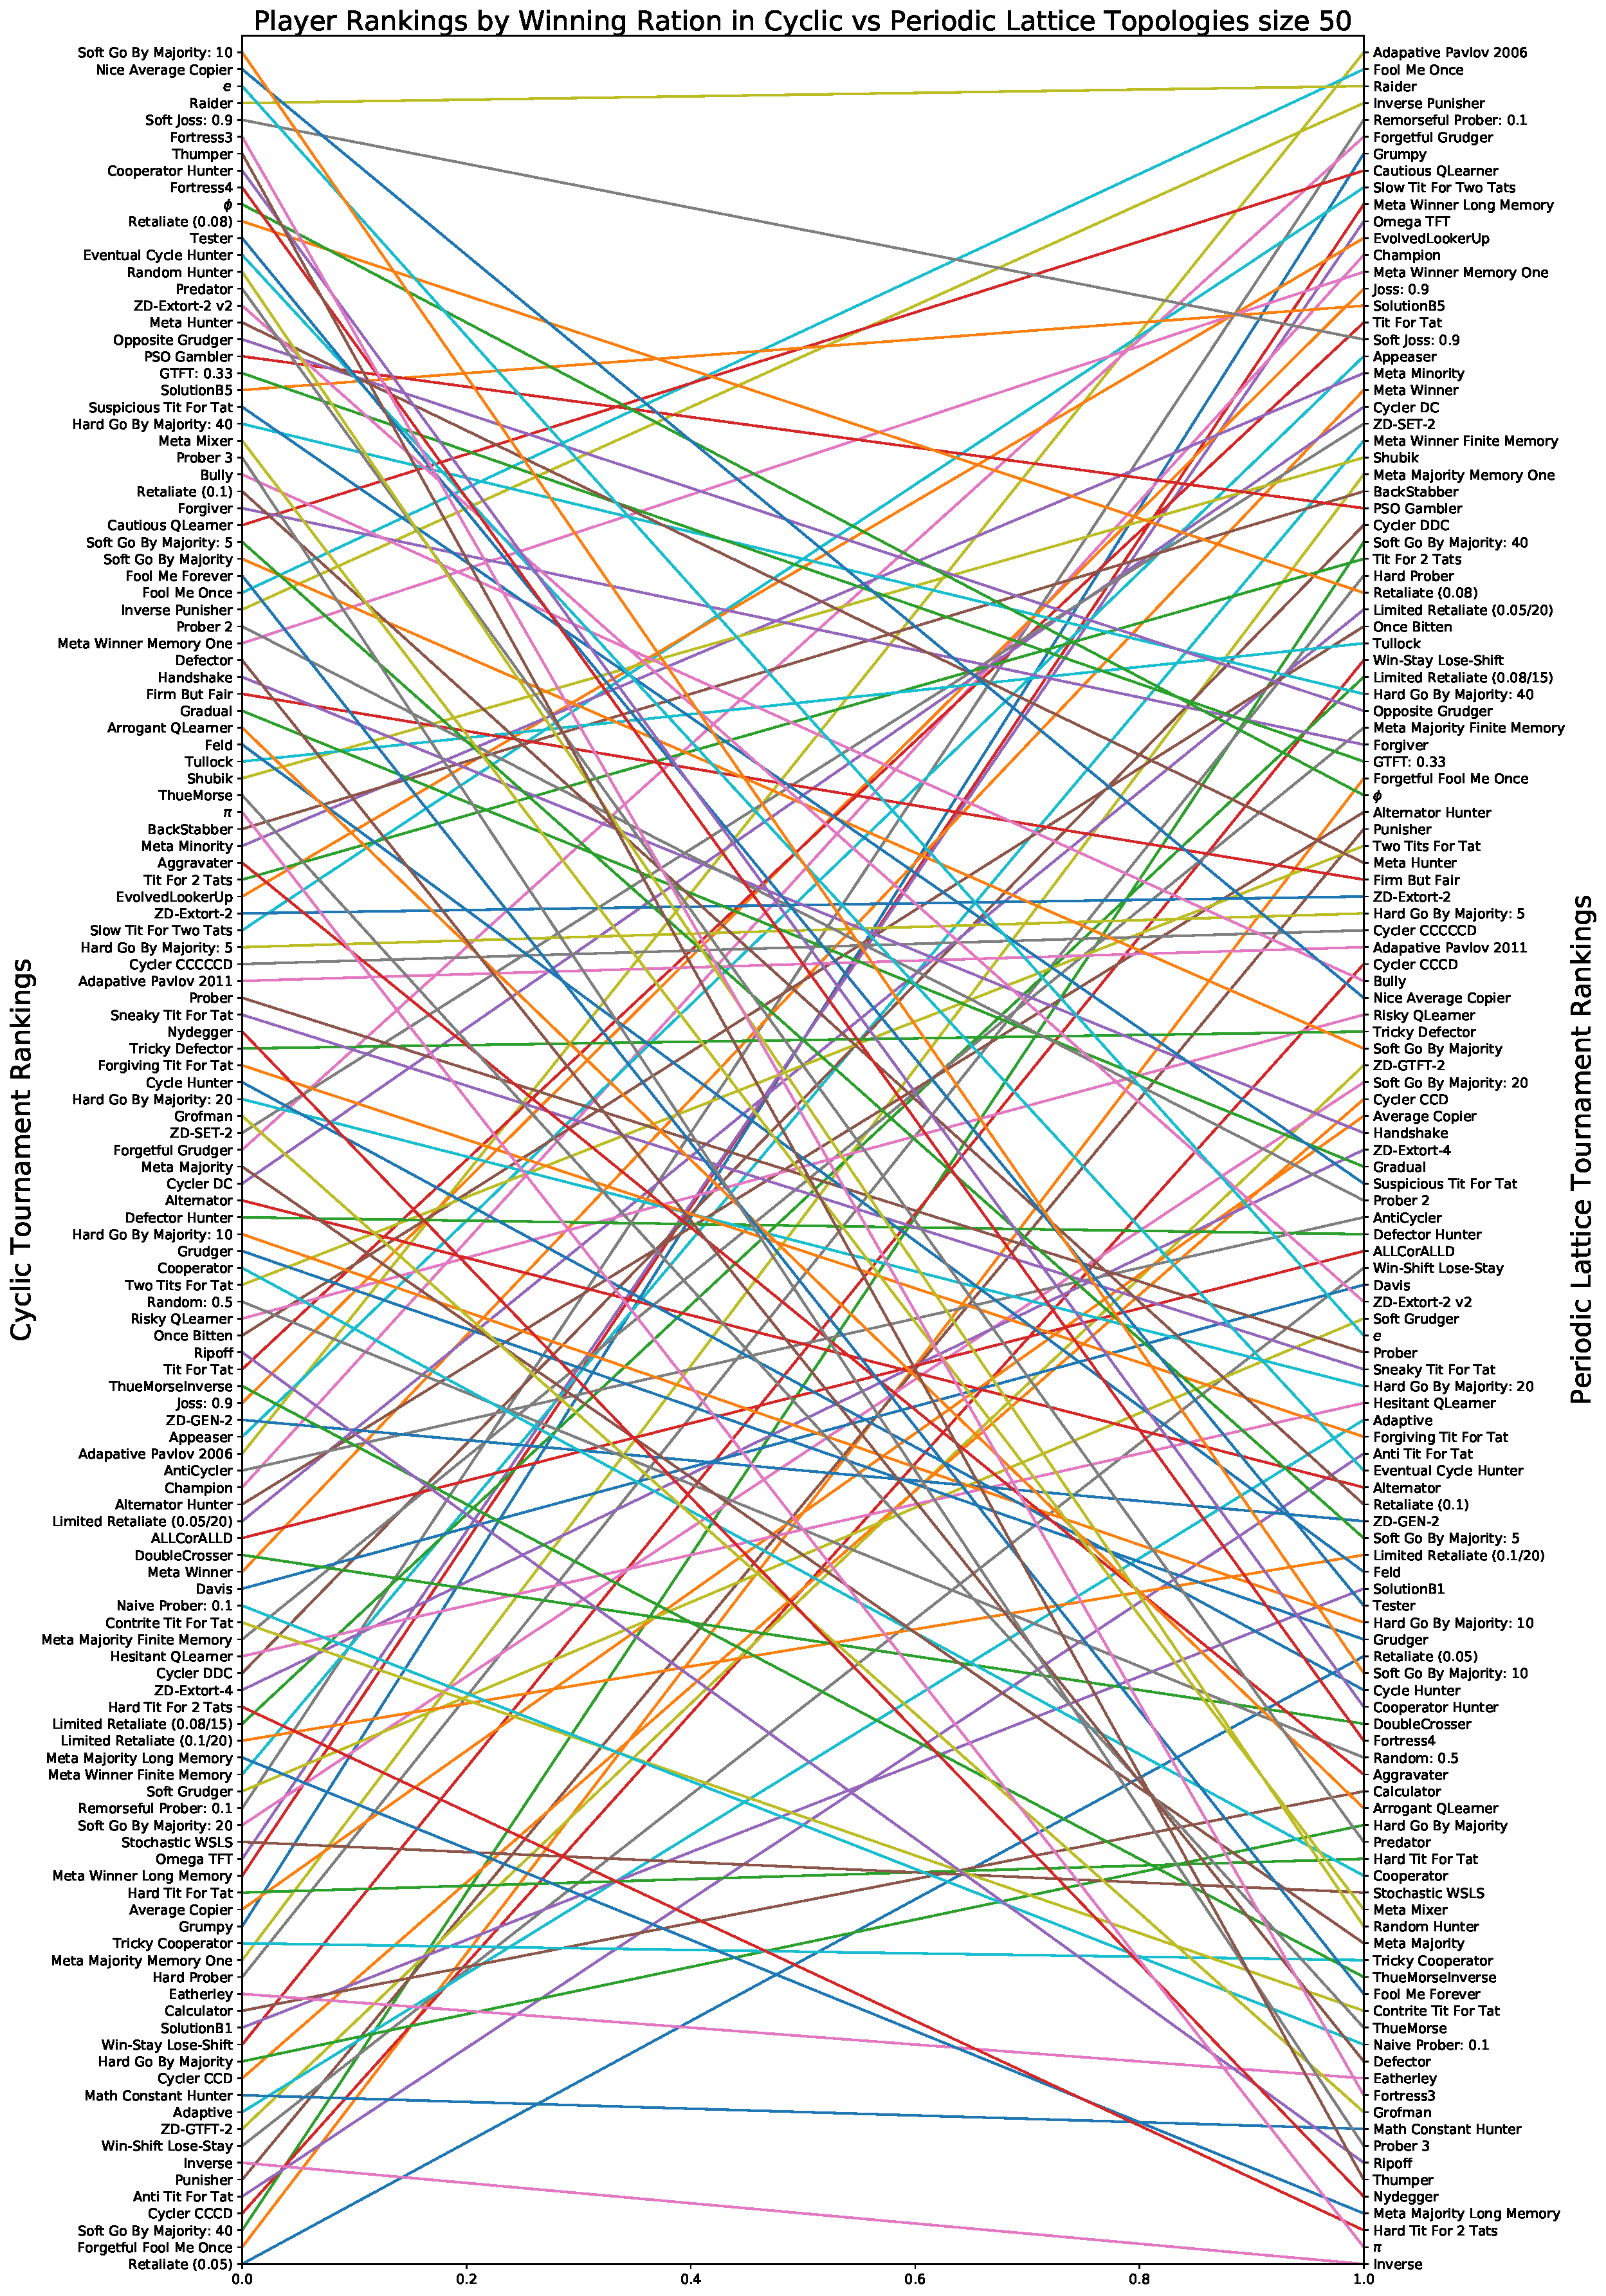
\includegraphics[width=0.55\linewidth]{static/winning_ratio.pdf}
	\end{center}
\end{frame}

\begin{frame}
	\begin{center}
		\huge{\textbf{}}\\~\\
		\small{@NikoletaGlyn}\\
		\small{https://github.com/Nikoleta-v3}\\
		\small{https://github.com/Axelrod-Python/Axelrod}
	\end{center}
\end{frame}

\end{document}
